\begin{frame}{}
    \LARGE Diffusion Models: \textbf{Forward Process}
\end{frame}

\begin{frame}[allowframebreaks]{Forward Diffusion Process}
    \begin{itemize}
        \item The forward process is a Markov chain that iteratively adds Gaussian noise to the image at each timestep.
        \item Given clean data $\mathbf{x}_0$, we generate $\mathbf{x}_t$ as:
        $$q(\mathbf{x}_t|\mathbf{x}_{t-1}) = \mathcal{N}(\mathbf{x}_t;\sqrt{1-\beta_t}\mathbf{x}_{t-1}, \beta_t\mathbf{I})$$
        \item Over many steps (e.g., 1000), the data becomes indistinguishable from pure noise.
    \framebreak
        \item This process is predefined and not learned.
        \item The full forward process:
        $$q(\mathbf{x}_{1:T}|\mathbf{x}_{0}) = \prod^{T}_{t=1}q(\mathbf{x}_t|\mathbf{x}_{t-1})$$
        \item Each new (slightly noisier) image at time step $t$ is drawn from a conditional Gaussian distribution with $\mathbf{\mu}_t = \sqrt{1 - \beta_t} \mathbf{x}_{t-1}$ and $\sigma^2_t = \beta_t$, which we can do by sampling $\mathbf{\epsilon} \sim \mathcal{N}(\mathbf{0}, \mathbf{I})$ and then setting $\mathbf{x}_t = \sqrt{1 - \beta_t} \mathbf{x}_{t-1} +  \sqrt{\beta_t} \mathbf{\epsilon}$.
    \end{itemize}
    \framebreak
    \begin{figure}
        \centering
        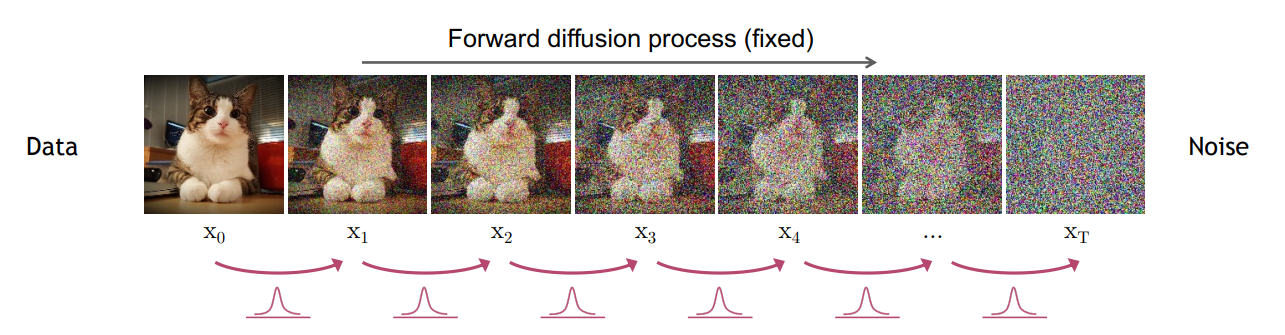
\includegraphics[height=0.7\textheight, width=\textwidth, keepaspectratio]{images/diffusion/diff_2.png}
    \end{figure}
    \begin{itemize}
        \item What if we want to go directly from $q_0$ to $q_t$?
        \item Let $\overline{\alpha}_t = \prod^t_{s=1}(1-\beta_s)$, then
        $$q(\mathbf{x}_t | \mathbf{x}_0) = \mathcal{N}(\mathbf{x}_t; \sqrt{\overline{\alpha}_t} \mathbf{x}_0 , (1 - \overline{\alpha}_t) \mathbf{I})$$
        \item This allows us, during training, to optimize random terms of the loss function $L$ (i.e., randomly sample $t$ and optimize $L_t$).
    \end{itemize}
\end{frame}

